In this section, we show that CopulaCPTS produces more calibrated and efficient confidence regions compared to existing methods on two synthetic datasets and two real-world datasets. We also demonstrate that CopulaCPTS's advantage is more evident over longer prediction horizons. We also show its effectiveness in the autoregressive prediction setting.

\paragraph{Baselines.} We compare our model with three representative works in different paradigms of uncertainty quantification for neural network time \edit{series} prediction: the Bayesian-motivated Monte Carlo dropout RNN (MC-dropout) by \cite{gal2016dropout}, the frequentist blockwise jackknife RNN (BJRNN) by \cite{bjrnn}, and a conformal forecasting RNN (CF-RNN) by \cite{Schaar2021conformaltime}. We use the same underlying prediction model for post-hoc uncertainty quantification methods BJRNN, CF-RNN, and CopulaCPTS. The MC-dropout RNN is of the same architecture but is trained separately, as it requires an extra dropout step during training and inference. 
%We also compare CF-RNN and CopulaCPTS with an encoder-decoder neural network model as the underlying predictor, to showcase the versatility and robustness of our algorithm. We denote these models as CF-\{\texttt{model name}\}, and copula-\{\texttt{modle name}\}.

\paragraph{Metrics.}
We evaluate calibration and efficiency for each method. For calibration, we report the empirical coverage on the held-out test set. Coverage should be as close to the desired confidence level $1-\alpha$ as possible. Coverage is calculated as $coverage_{1-\alpha} =  \mathbb{E}_{x,y \sim \mathbf{X} \edit{\times} \mathbf{Y}} P(\mathbf{y} \in \Gamma^{1-\alpha}(\mathbf{x})) \approx \frac{1}{n} \sum^n_1 \mathbbm{1} (\mathbf{y}_n \in \Gamma^{1-\alpha}_n(\mathbf{x}_n)\edit{)}$. For efficiency, we report the average area (2D) or volume (3D) of the confidence region. The metric should be as small as possible while being valid (coverage maintains above pre-specified confidence level). The area or volume is calculated as $area_{1-\alpha} = \mathbb{E}_{x \sim \mathbf{X}} \|\Gamma^{1-\alpha}(x)\|  \approx \frac{1}{n} \sum^n_1 \|\Gamma^{1-\alpha}(x_n)\|$.


\subsection{Synthetic Datasets}

We first test the effectiveness of our models with two synthetic spatiotemporal datasets - interacting particle systems \edit{\cite{nridataset}}, and drone trajectory following (simulated with PythonRobotics \edit{\cite{pythonrobotics}}). For the particle simulation we predict $\mathbf{y}_{t+1:t+h}$ where $t=35$, $h=25$ and $y_t \in \mathbb{R}^2$; for drone simulation $t=60$, $h=10$, and $y_t \in \mathbb{R}^3$. To add randomness to the tasks, we added Gaussian noise of $\sigma = .01$ and $.05$ to the dynamics of the particle simulation, and $\sigma = .02$ to drone dynamics. \edit{We generate 5000 samples for each dataset, and split the data by 45/45/10 for train, calibration, and test respectively. Please see Appendix C.1 for forecaster model details.}

We visualize the calibration and efficiency of the methods in \autoref{fig:synthetic} for confidence levels $1-\alpha = 0.5$ to $0.99$. We can see that Copula-RNN, the red lines, are more calibrated and efficient compared to other baseline methods, especially in tasks with large noise (particle dataset, $ \sigma = 0.05$). We can see that for harder tasks (particle $ \sigma = 0.05$, and drone trajectory prediction), MC-Dropout is overconfident, whereas BJ-RNN and CF-RNN produce very large (hence inefficient) confidence regions. This behavior of CF-RNN is expected because they apply Bonferroni correction to account for joint prediction for multiple time steps, which is an upper bound of copula functions. The numbers for confidence level $90\%$ are presented in Table \ref{tab:baselines_new}. A quantitative comparison of confidence regions for drone simulation can be found in Figure \ref{fig:drone} in the appendix.

\begin{figure}[h]
    \centering
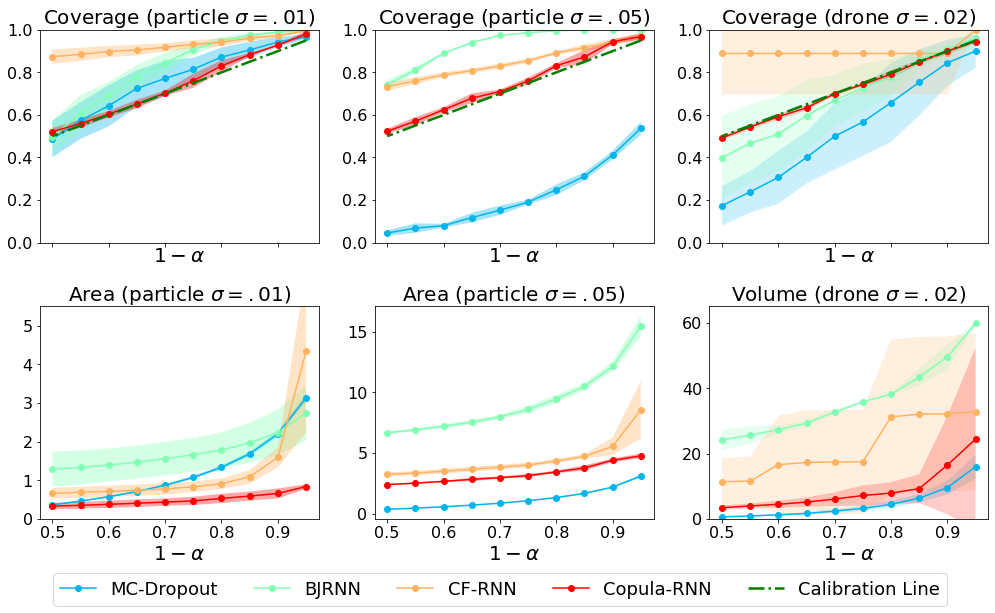
\includegraphics[width=0.9\linewidth]{copula/figs/synthetic_update.png}
    \caption{Calibration (upper row) and efficiency (lower row) comparison on different $1-\alpha$ levels for simulated data sets. For calibration, the goal is to coincide with the green dotted calibration line as closely as possible while staying valid (above the green line). Note that copula methods are more calibrated across different significance levels. For efficiency, we want the metric to be as low as possible. Copula-RNN outperforms the baselines consistently. (MC-dropout for the right two experiments produces invalid regions, so we don't consider its efficiency.)}
    \label{fig:synthetic}
\end{figure}


% ---------------------------------
% updated table
% ---------------------------------
\begin{table}
\centering
\begin{tabular}{ c | c | c  c c  c  } 
 \toprule
 & & MC-dropout & BJRNN & CF-RNN & Copula-RNN \\
\midrule\midrule
 \multirow{2}{*}{\begin{tabular}{l}Particle Sim \\ ($\sigma=.01$)\end{tabular}} & Coverage  & \color{gray}{  63.9 \plusminus 16.1  } &   98.9 \plusminus 0.2   &   97.0 \plusminus 2.3   & \textbf{  91.5 } \plusminus 2.1   \\ 
 & Area  & \color{gray}{  0.81 \plusminus 0.05  } &   2.24 \plusminus 0.59   &   3.13 \plusminus 3.24   &  \textbf{1.06}  \plusminus 0.36   \\ \midrule  
 \multirow{2}{*}{\begin{tabular}{l}Particle Sim\\ ($\sigma=.05$)\end{tabular}} & Coverage  & \color{gray}{  16.1 \plusminus 4.3  } &   100.0 \plusminus 0.0   &   94.5 \plusminus 1.5   & \textbf{  90.3} \plusminus 0.7   \\ 
 & Area  & \color{gray}{  0.79 \plusminus 0.02  } &   12.13 \plusminus 0.39   &   5.79 \plusminus 0.51  & \textbf{  4.50 } \plusminus 0.07   \\ \midrule  
 \multirow{2}{*}{\begin{tabular}{l}Drone Sim\\ ($\sigma=.02$)\end{tabular}} & Coverage  & \color{gray}{  84.5 \plusminus 10.8  } &   90.8 \plusminus 2.8   &   91.6 \plusminus 9.2   &  \textbf{90.0} \plusminus 1.5  \\ 
 & Volume  & \color{gray}{  9.64 \plusminus 2.13 } &   49.57 \plusminus 3.77  &   32.18 \plusminus 13.66  &  \textbf{16.52}  \plusminus 7.08  \\
 \midrule\midrule
 \multirow{2}{*}{\begin{tabular}{l}COVID-19 \\ Daily Cases \end{tabular}} & Coverage  & \color{gray}{ 19.1 \plusminus 5.1 } &  \color{gray}{ 79.2 \plusminus 30.8}  &  95.4 \plusminus 1.9  & \textbf{ 92.1} \plusminus 1.0  \\ 
 & Area  & \color{gray}{ 34.14 \plusminus 0.84  } &  \color{gray}{ 823.3 \plusminus 529.7}  &  610.2 \plusminus 96.0  & \textbf{429.0} \plusminus 15.1  \\   \midrule 
 \multirow{2}{*}{\begin{tabular}{l}Argoverse \\ Trajectory \end{tabular}} & Coverage  & \color{gray}{ 27.9 \plusminus 3.1 } &  92.6 \plusminus 9.2  &  98.8 \plusminus 1.9  &  \textbf{90.4} \plusminus 0.3 \\ 
 & Area  & \color{gray}{ 127.6 \plusminus 20.9 } &  880.8 \plusminus 156.2  &  396.9 \plusminus 18.67  &  \textbf{126.8} \plusminus 12.22 \\  
\bottomrule
\end{tabular}
\caption{Performance on synthetic and real world datasets with target confidence $1-\alpha = 0.9$. Methods that are \textit{invalid} (coverage below $90\%$) are greyed out. CopulaCPTS achieves high level of calibration (coverage is close to $90\%$) while producing more efficient confidence regions (small area).} 
\label{tab:baselines_new}
\end{table}


% ---------------------------------
% real world dataset
% ---------------------------------

\subsection{Real world datasets}
%We choose two scenarios in the real world where calibrated and sharp uncertainty quantification are important. 

\textbf{COVID-19.} We replicate the experiment setting of \cite{Schaar2021conformaltime} and predict new daily cases of COVID-19 in regions of the UK. The models take 100 days of data as input and forecast 50 days into the future. We used 200 time series for training, 100 for calibration, and 80 for testing.

\textbf{Vehicle trajectory prediction.} The Argoverse autonomous vehicle motion forecasting dataset \cite{argoverse} is a widely used vehicle trajectory prediction benchmark. The task is to predict 3 second trajectories based on all vehicle motion in the past 2 seconds sampled at 10Hz. Because trajectory prediction is a challenging task, we utilize a state-of-the-art prediction algorithm LaneGCN \cite{liang2020learning} as the underlying model for CF-RNN and Copula-RNN \edit{(details in Appendix C.1)}. Flexibility of underlying forecasting model is an advantage of post-hoc conformal prediction methods. \edit{For model-dependent baselines MC-dropout and BJRNN, we have to train an RNN forecasting model from scratch for each method, which is additional computational cost.} 
%We re-train an encoder-decoder RNN model for MC-dropout and BJRNN which are more computationally heavy.

Results in Table \ref{tab:baselines_new} show that, like for synthetic datasets,  CopulaCPTS is both more calibrated and efficient compared to baseline models for real world datasets. For the trajectory prediction task, learning the copula results in a $77\%$ sharper confidence region while still remaining valid for the $90\%$ confidence interval. We visualize two samples from each dataset in Figure \ref{fig:realworld}.
The importance of efficiency in these scenarios is clear - the confidence regions need to be narrow enough for them to be useful for decision making. Given the same underlying prediction model, we can see that CopulaCPTS produces a much sharper region while still remaining valid.

\begin{figure}
\centering
\begin{subfigure}{.245\textwidth}
  \centering
  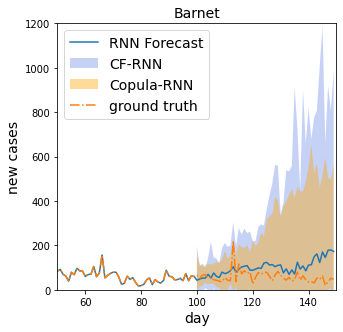
\includegraphics[width=\linewidth]{copula/figs/covidnew1.png}
  \label{fig:cov001}
\end{subfigure}%
\begin{subfigure}{.245\textwidth}
  \centering
  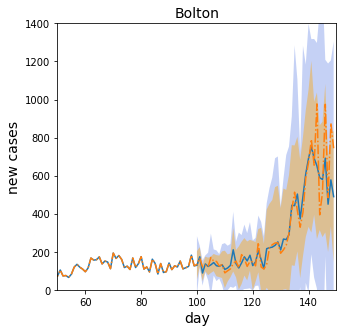
\includegraphics[width=\linewidth]{copula/figs/covidnew2.png}
  \label{fig:cov002}
\end{subfigure}
\begin{subfigure}{.245\textwidth}
  \centering
  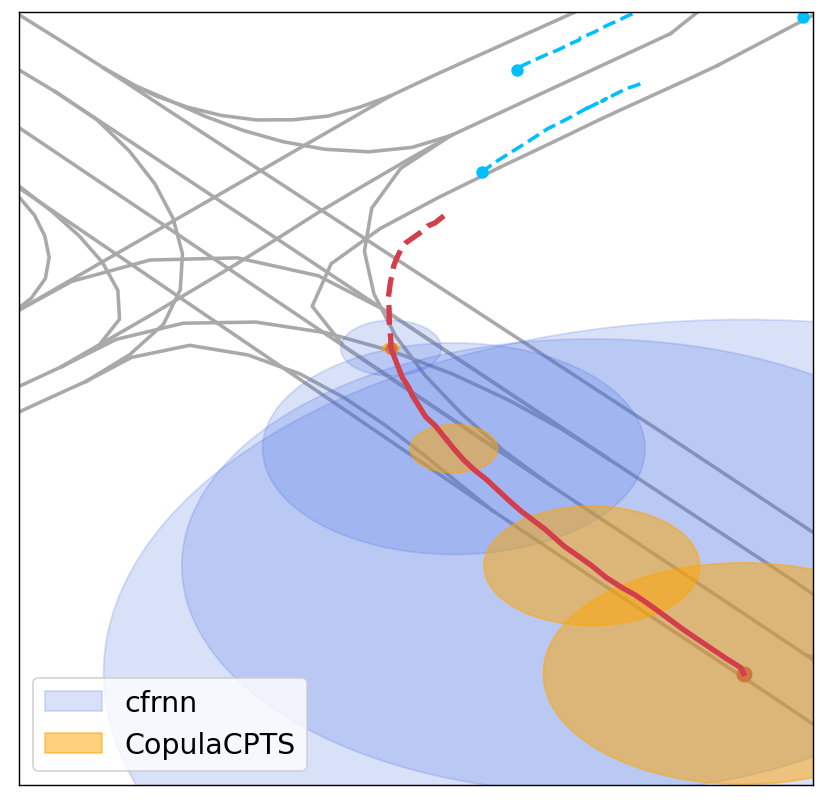
\includegraphics[width=\linewidth]{copula/figs/argoverse1.png}
  \label{fig:conf1}
\end{subfigure}%
\begin{subfigure}{.245\textwidth}
  \centering
  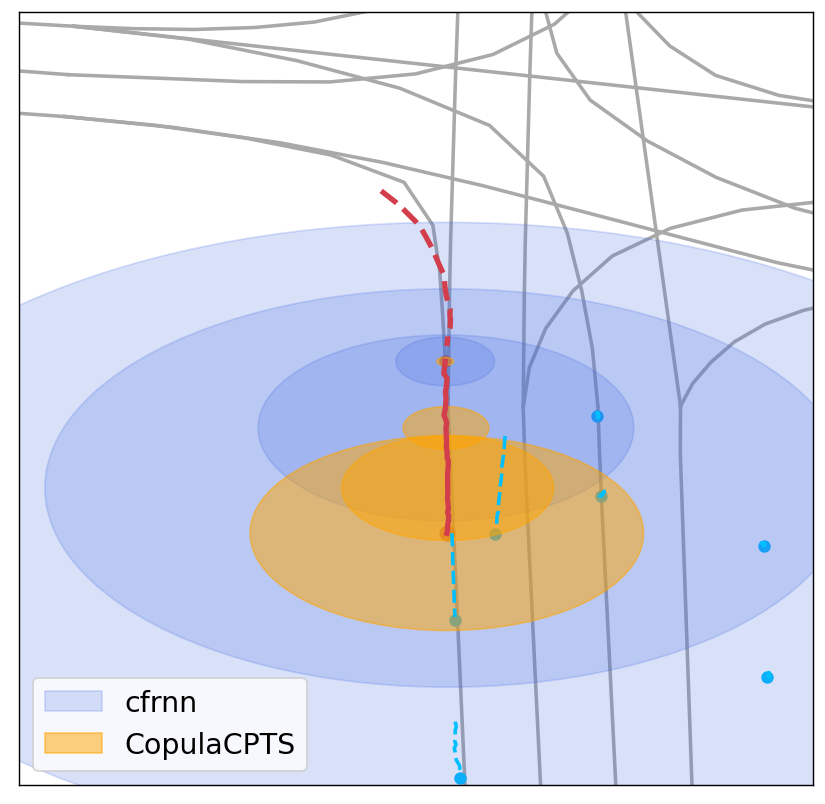
\includegraphics[width=\linewidth]{copula/figs/argoverse2.png}
  \label{fig:conf2}
\end{subfigure}
\caption{Illustrations of 90\% confidence regions given by CF-RNN (blue) and CopulaCPTS (orange) on two real-world datasets. For COVID-19 forecast (left 2) we see that CopulaCPTS produces sharper yet covering confidence regions. For Argoverse (right 2) we illustrate regions at time steps 1, 10, 20, and 30. Note that the confidence region produced CF-RNN is uninformatively large, as it covers all the lanes. Overall, CopulaCPTS is able to produce much more efficient confidence regions while maintaining valid coverage. These examples also  illustrate the importance of efficiency.}
\label{fig:realworld}
\end{figure}

\paragraph{Comparison of models at different horizon lengths.} CopulaCPTS is an algorithm designed to produce calibrated and efficient confidence regions for multi-step time series. When the prediction horizon is long, CopulaCPTS's advantage is more pronounced. Figure \ref{fig:horizon} shows performance comparison across increasing time horizons on the particle dataset. See Table \ref{tab:baselines} of Appendix \ref{app:exp_details} for additional experiment results. CopulaCPTS achieves a $30\%$ decrease in area at 20 time steps compared to CF-RNN, the best performing baseline; the decrease is above $50\%$ at 25. This experiment shows significant improvement of using copula to model the joint distribution of future time steps. 

\paragraph{CopulaCPTS for the Autoregressive prediction setting.} We test the autoregressive setting (section 4.3) on the COVID-19 dataset. We train an RNN model with $k=7$ and use it to autoregressively forecast the next 14 steps. Table \ref{tab:autoregressive} compares the performance of re-estimating the copula for each 7-step forecasts versus using a fixed copula calibrated using the first 7 steps. We compare the model to a 14-step joint forecaster using CopulaCPTS as well.  

\begin{figure}
    \centering
    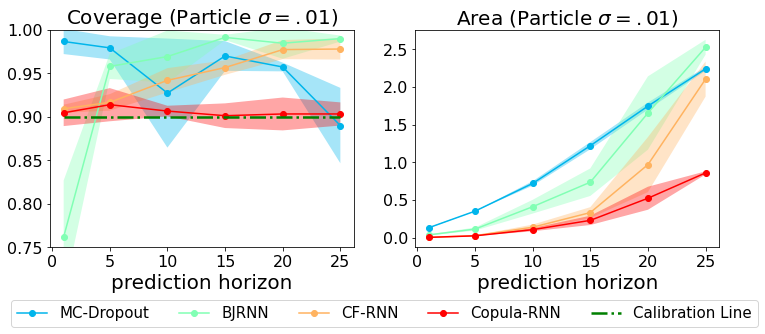
\includegraphics[width=0.6\textwidth]{copula/figs/horizon01.png}
\captionof{figure}{CopulaCPTS remains more calibrated and efficient than baselines over increasing forecast horizons.}
\label{fig:horizon}
\end{figure} 

\begin{table}
    \centering
    \begin{tabular}{c|c|c}
    \toprule
    Method & Coverage & Area \\
          \midrule\midrule
    AR re-estimate  & \textbf{90.7}  & \textbf{377.9} \\
    AR fixed  & 88.2  & 340.5 \\
    Joint & 90.8 & 429.4\\
         \bottomrule
    \end{tabular}
    \captionof{table}{Performance of autoregressive (AR) CopulaCPTS.  Re-estimating copula gives us valid confidence region over time and is more efficient than joint CopulaCPTS forecast.}
    \label{tab:autoregressive}
\end{table} 


